\chapter{EXPERIMENTOS E RESULTADOS OBTIDOS}
\label{c.Desenvolvimento}

O desenvolvimento do projeto dividiu-se em quatro fases: a montagem do ambiente
de testes de assinaturas construídas a partir de regras do Yara; a obtenção das
regras e construção de um índice de agrupamento das mesmas para agilizar a
execução das varreduras; obtenção e escolha de amostras de \textit{malware} para
testagem; bateria de testes final e análise de resultados. Complementarmente,
foi desenvolvida a ideia de uma aplicação \textit{web} para análise de
\textit{malware} com base em regras de detecção do Yara.

\section{Obtenção das regras de detecção e das amostras de \textit{malware}}
\label{s.obtregras}

A primeira etapa da implementação computacional do projeto é composta da
construção de um índice de regras do Yara compilado a partir das bases de
assinaturas do ClamAV e de outros conjuntos avulsos e menores de assinaturas
disponibilizados em repositórios de código aberto; em paralelo, também
construiu-se um conjunto de algumas amostras ``vivas'' e selecionadas de
\textit{malware} para a testagem do índice sobre arquivos infectados. Foram
selecionadas apenas amostras de \textit{malware} `potencialmente inofensivo',
como \textit{trojans}, que dependem de um comando de execução disparado por um
usuário descuidado, para que não houvesse risco de propagação e infecção do
próprio ambiente local e de redes com as quais o ambiente local se comunicasse.
Por isso, com intuito de prevenção, optou-se pela não realização de testes em,
por exemplo, \textit{worms}, que são capazes de propagarem-se de maneira
independente pelos ambientes onde chegam. Para converter as assinaturas, foi
adaptado um \textit{script} em Python que interpreta os arquivos no que contém
as assinaturas do ClamAV, cujo formato é .cvd, e reescreve-as na sintaxe
amigável de regras do Yara com a utilização de expressões regulares. Na figura
8 ilustra-se o funcionamento do \textit{script} descrito envolvendo as
bases de dados utilizadas na implementação:
% TODO: SCREENSHOT DO SCRIPT DE CONVERSÃO FUNCIONANDO
\begin{figure}[H]
  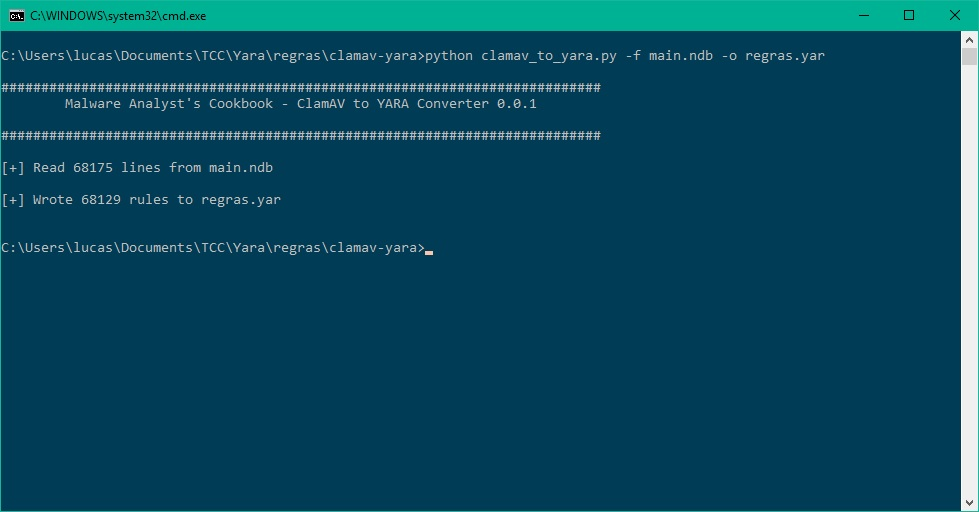
\includegraphics[scale=0.6]{figs/regras_convertidas}
  \centering
  \caption{Funcionamento do \textit{script} de conversão de bases do ClamAV para regras do Yara}
  \label{f.regras_convertidas}
  \legend{Fonte: Elaborada pelo autor.}
\end{figure}

Após a tradução das regras contidas nas bases de dados, é necessário compilá-las
antes de finalmente ser possível aplicá-las numa varredura real. Um outro
pequeno \textit{script} em Python é capaz de realizar essa tarefa, vide
código-fonte exibido na figura 9:
\begin{figure}[H]
  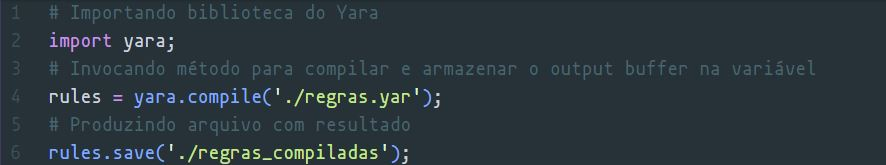
\includegraphics[scale=0.6]{figs/script_conversao}
  \centering
  \caption{Script para compilação das regras de detecção}
  \label{f.script_comp}
  \legend{Fonte: Elaborada pelo autor.}
\end{figure}

No final desta seção do texto, há uma lista com os \textit{links} para
\textit{download} de todo o código-fonte utilizado na implementação do projeto.

\section{Testes iniciais com o ambiente de desenvolvimento}
\label{s.testesiniciais}

Apenas com a finalidade de atestar o funcionamento da ferramenta estudada no
projeto, antes de decidir seguir com seu uso no decorrer da implementação
planejada, algumas regras de teste simples foram aplicadas sobre alguns arquivos
de texto contendo pedaços de código e um conjunto de \textit{strings} que
deveria ser descoberto numa varredura. Os testes foram bem sucedidos nesta etapa
por dois motivos; primeiro, as regras escritas eram pequenas e rudimentares, e
em segundo lugar também ainda não havia necessidade de conversão de bancos de
assinaturas ou montagem de índices mais complexos e adaptação de
\textit{scripts} envolvidos neste processo inicial. Numa tentativa mais
condizente com um cenário real de detecção de \textit{malware}, se fez a
construção de um índice com um número bem maior de regras obtidas nos
repositórios já citados previamente. Contudo, nesta segunda etapa ainda não
houve tentativa de converter as regras contidas dentro das bases de assinaturas do
ClamAV, por motivos de complexidade e de completude dos testes propostos. Nessa
mesma fase, as regras foram aplicadas dentro de um conjunto mais numeroso de
arquivos, já contendo alguns arquivos de código-fonte e também executáveis de
\textit{malware} misturados em algumas pastas, para ver como o Yara funcionaria
num contexto de varredura mais recursivo. Estas duas primeiras etapas de testes
foram bem sucedidas e o Yara acusou corretamente quais arquivos continham as
características mapeadas pelas assinaturas do índice de regras aplicado.



\section{Testagem completa e análise de resultados}
\label{s.testefull}

Para consolidar o trabalho com a ferramenta de uma maneira mais definitiva, um
conjunto de aplicativos ``saudáveis'' foi misturado com as amostras de
\textit{malware}, e depois espalhado arbitrária e aleatoriamente dentro de uma
estrutura de pastas para que se efetuasse uma varredura recursiva, utilizando um
índice de regras mais extenso, agora contendo as regras convertidas e compiladas
a partir das bases de dados do ClamAV e das demais regras avulsas encontradas
durante a pesquisa desenvolvida. A varredura foi bem sucedida e o Yara não
apontou falsos-positivos quando passou pelos arquivos limpos. A única
dificuldade encontrada foi quanto à varreduras envolvendo as regras de detecção
para \textit{malware} construído para dispositivos móveis, onde as regras
relacionadas ao sistema \textit{Android} procuravam importar módulos do
\textit{kit} de desenvolvimento do mesmo, que não estava instalado no ambiente
do projeto, gerando tal problema que por questões de \textit{hardware} não foi
contornado, pois o carregamento de toda a estrutura do \textit{kit}
sobrecarregava os recursos disponíveis na implementação,  tornando inviáveis os
testes envolvendo esse grupo de regras. Contudo, na possibilidade de continuar o
desenvolvimento do projeto num ambiente com \textit{hardware} mais generoso e
com o uso de um sistema operacional mais apropriado para esse tipo de trabalho,
pode-se afirmar com segurança que as regras funcionariam sem nenhum problema.
Enfim, o resultado da varredura recursiva envolvendo um índice de regras
completo foi satisfatório e  esclarecedor quanto ao funcionamento e à
confiabilidade da ferramenta estudada.

\section{Aplicação web}
\label{s.prototipo}

Foi elaborada a ideia de uma aplicação capaz de receber regras do Yara ou
arquivos de bases de assinaturas de \textit{malware} para manter sua própria
base de dados unificada e também capaz de realizar varreduras em arquivos
carregados pelos usuários ao servidor da aplicação. Na figura 10 temos um
esboço dos elementos e do funcionamento da aplicação projetada.

\begin{figure}[H]
  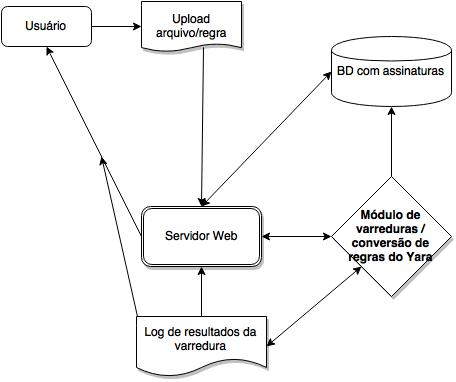
\includegraphics[scale=0.6]{figs/flux_prototipo}
  \centering
  \caption{Fluxograma de funcionamento da aplicação.}
  \label{f.flux_prototipo}
  \legend{Fonte: elaborada pelo autor.}
\end{figure}

Trabalhou-se também numa possível estrutura de comunicação entre os módulos
utilizando os recursos de uma API \textit{RESTful}, que cobriria as funções de
transação com o banco de dados, execução de scripts na camada do servidor e de
\textit{upload} e devolução de arquivos entre clientes e servidor, como por
exemplo o recente projeto Laravel PHP. Pode-se sugerir que A API troque dados
com um \textit{front-end} implementado em cima do \textit{framework} Angular JS,
atualmente disponível em sua segunda versão, pelas facilidades que ele contém
para o desenvolvimento de aplicações que possuem arquitetura semelhante à
apresentada na ideia descrita. Foi decidido o emprego de tais tecnologias nessa
implementação pois são ótimas para se trabalhar com processamento interno de
arquivos de texto, por já incluirem bibliotecas para tratamento e interpretação
de arquivos respeitando diversos parâmetros para combinação e verificação de
\textit{strings} sob padrões e expressões regulares, que auxiliariam muito na
automatização dos processos de formatação e validação dos arquivos, com a
finalidade de assegurar o funcionamento correto da montagem dos índices de
regras contendo assinaturas e dos \textit{scripts} de varredura de arquivo
executados na camada do servidor.

\section{Repositório do projeto no GitHub}
\label{s.repositorio}
Como dito anteriormente, o projeto foi centralizado e disponibilizado num
repositório \textit{online} dentro do \textit{GitHub} para versionamento de
código e também do desenvolvimento da monografia. Todo o material utilizado na
implementação do projeto encontra-se lá também disponível para
\textit{Download}. O endereço se encontra na seção de conclusão da monografia.
